
\section{Calculations \& Graphs}

\vspace{-0.5cm}
\singlespacing

%------- AVERAGE VALUE --------%

\subsection{Average Value Formula} 

\begin{align*}
		\overline{a} = \frac{sum\,of\,values}{total\, \#\,of\,values} 
\end{align*}

\subsubsection{Sample Calculation \\ {\normalfont \small\textit{average acceleration of free fall trials}}}

\begin{align*}
	\overline{a} & = \frac{9.751 + 9.758 + 9.749 + 9.620 + 9.769 + 9.837}{6} \\
							 &= \boxed{9.747\thinspace m/s^2}
\end{align*}

%------- AVERAGE VALUE --------%

%------- STANDARD DEVIATION --------%
\subsection{Standard Deviation Formula}

\begin{align*}
		\sigma &= \sqrt{\frac{\Sigma(x_i -\overline{a})^2}{N}} \\
		 &= \sqrt{\frac{SS}{N}} \\ \\
		\textbf{N} &:\, \text{Total number of values} \\
		\overline{\textbf{a}} &:\, \text{Average value} \\
		\textbf{x\textsubscript{i}} &:\, \text{Each value from the data set} \\
		\textbf{SS} &:\, \text{Sum of squares} 
\end{align*}

\subsubsection{Sample Calculation \\ {\normalfont \small\textit{std of free fall trials}}}

\begin{align*}
	\sigma &= \sqrt{\frac{(9.751-\overline{a})^2 + ... + (9.837-\overline{a})^2}{6}} \\
		 &= \sqrt{\frac{0.024865333}{6}} \\
		 &= \boxed{0.06439\thinspace m/s^2}
\end{align*}
%------- STANDARD DEVIATION --------%

%------- RELATIVE ERROR --------%
\subsection{Relative Error Formula}

\begin{align*}
	RE &= \left| {\frac{V_A-V_E}{V_E}} \right|\: \text{x}\: 100\% \\ \\
	\boldsymbol{V_A} &:\, \text{Actual value observed} \\
	\boldsymbol{V_E} &:\, \text{Expected value} 
\end{align*}

\subsubsection{Sample Calculation \\ {\normalfont \small\textit{acceleration of free fall trial 1}}}

\begin{align*}
	RE &= \left| {\frac{9.751-9.80}{9.80}} \right|\: \text{x}\: 100\% \\
			&= \boxed{0.4917\%} 
\end{align*}
%------- RELATIVE ERROR --------%

\subsection{Free Fall}

\subsubsection{Trial 1}
%----FF TRIAL 1-----%
\begin{table}[H]
\centering
\begin{tabular}{@{}cc@{}}
\toprule
\textbf{Time(s)} & \textbf{Velocity(m/s)} \\ \midrule
0.0532 & 1.199 \\
0.08952 & 1.553 \\
0.1189 & 1.841 \\
0.1444 & 2.087 \\
0.1671 & 2.31 \\
0.1878 & 2.513 \\ \midrule
\textbf{\begin{tabular}[c]{@{}c@{}}Average \\ Acceleration \\ ($\boldsymbol{m/s^2}$)\end{tabular}} & 9.751 \\ \bottomrule
\end{tabular}
\caption{Velocity vs Time | Free Fall Trial 1}
\label{tab:ff-t1}
\end{table}

\begin{figure}
	\begin{center}
		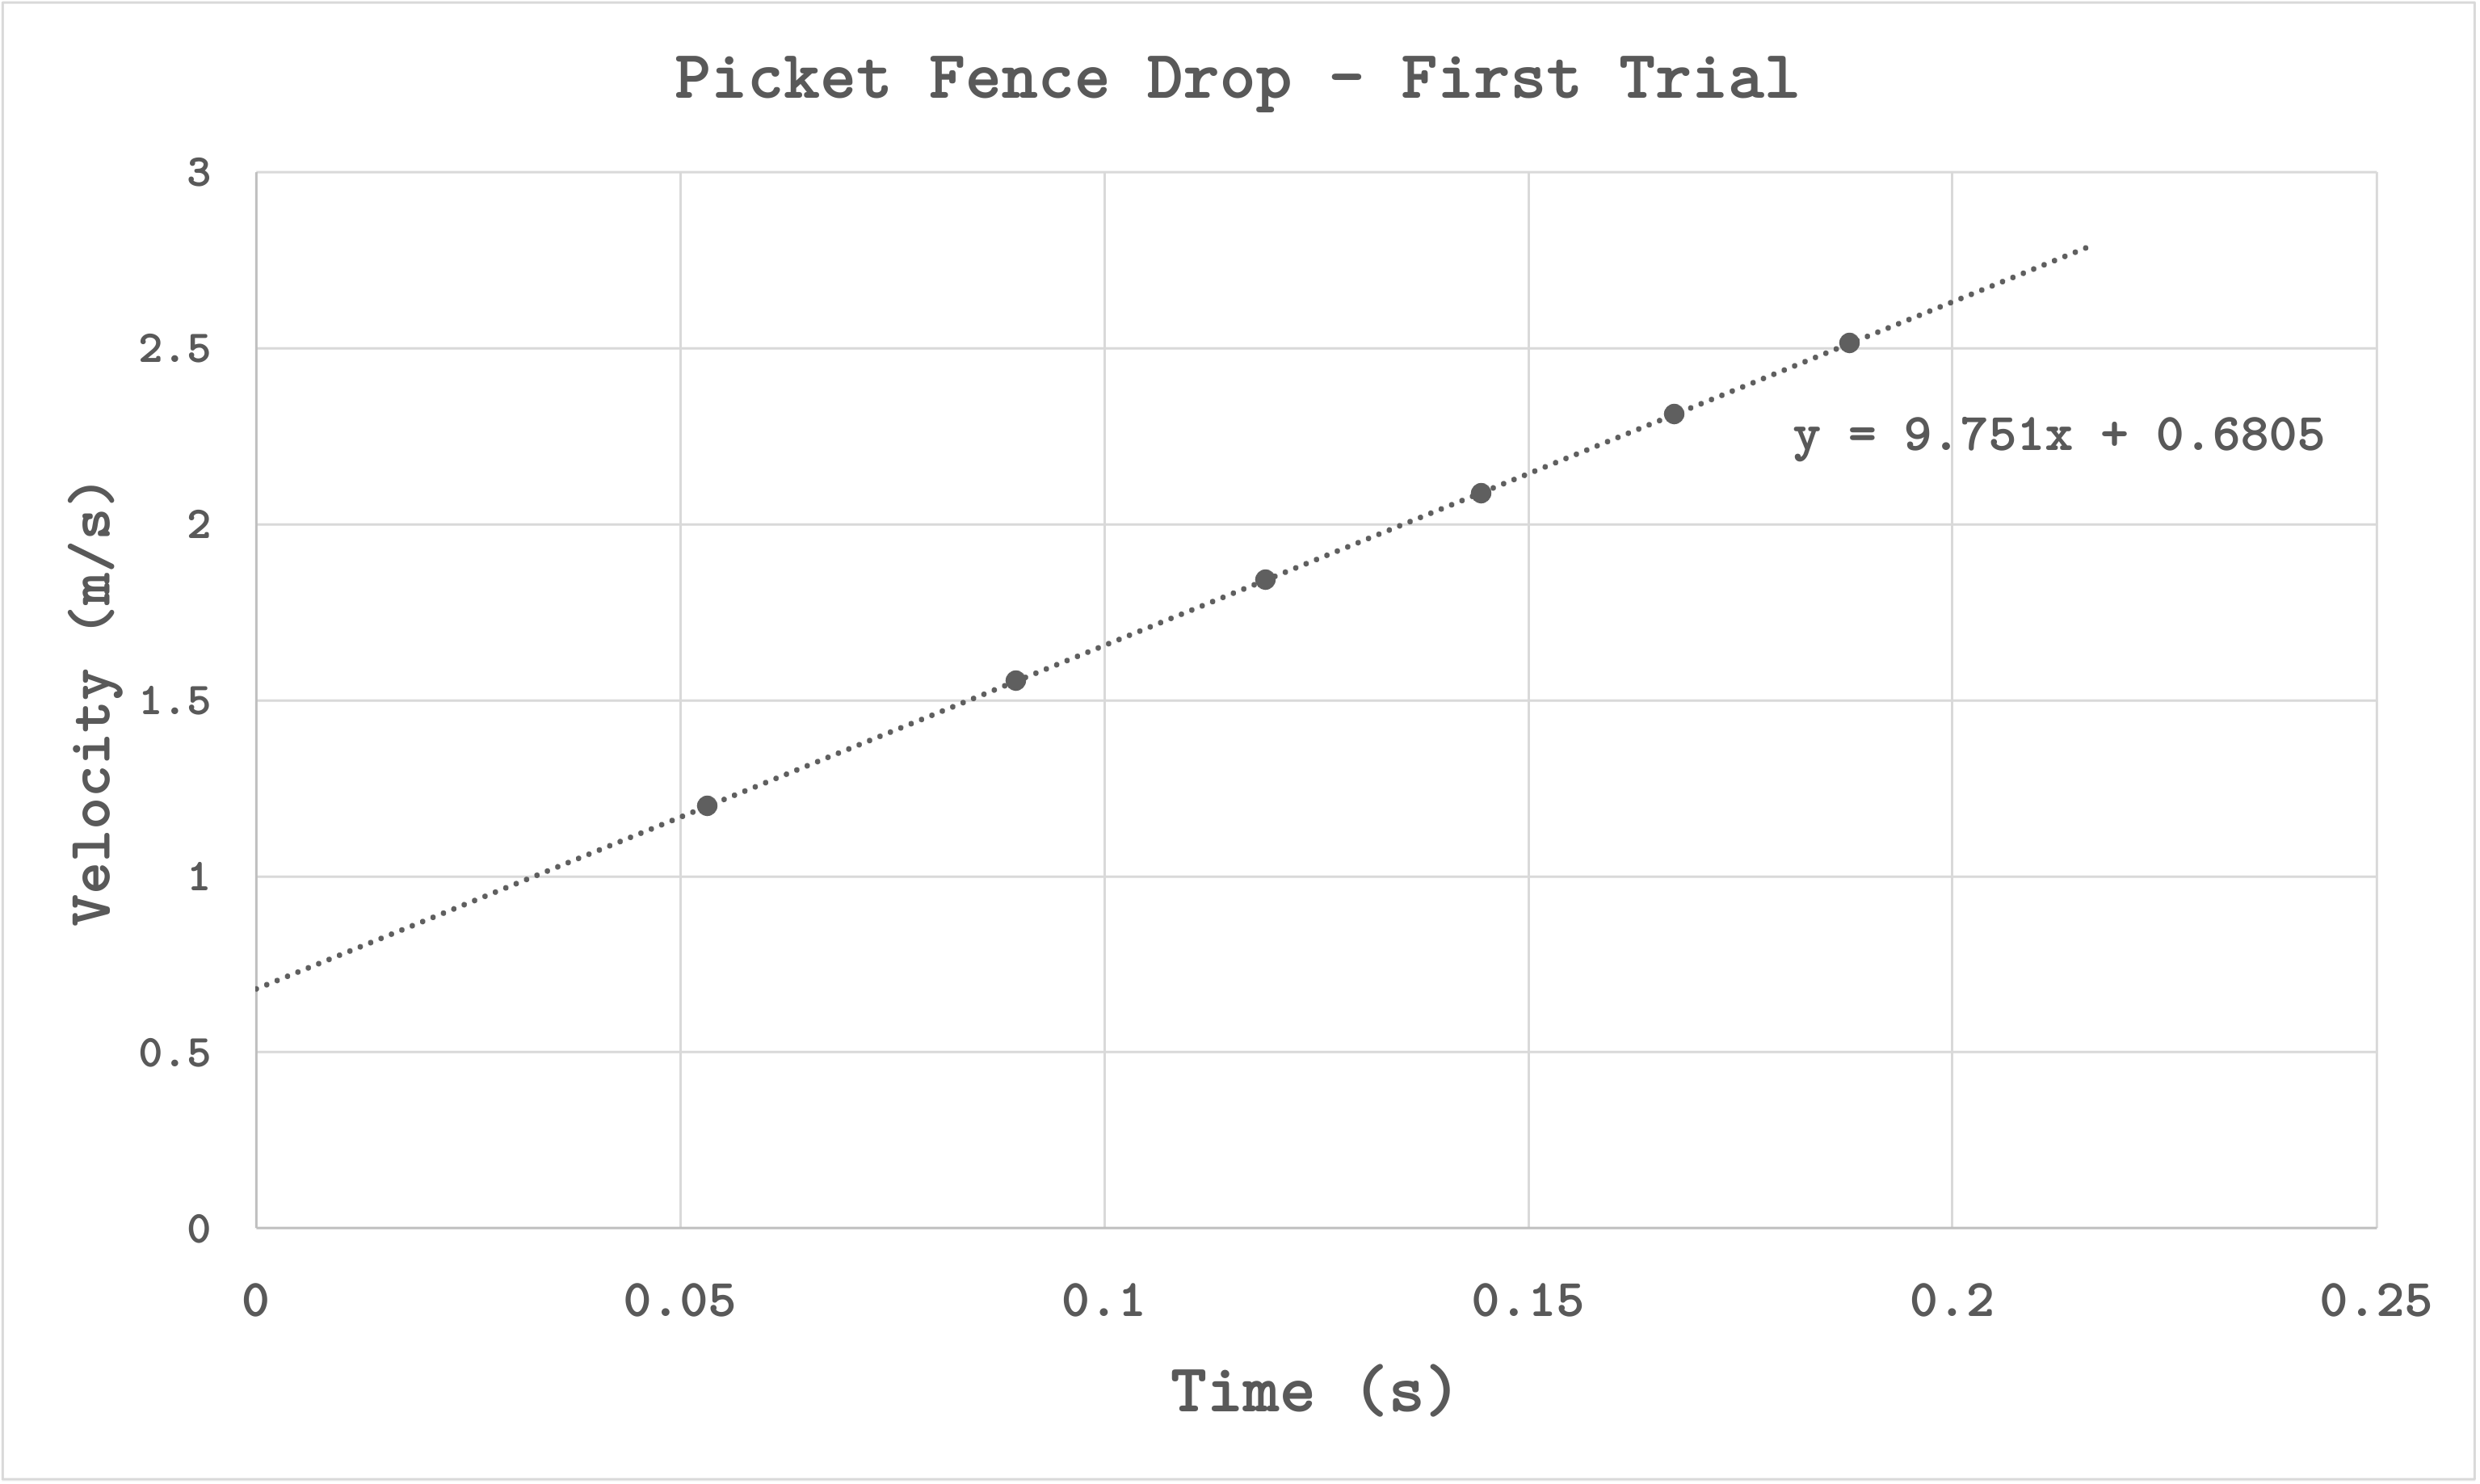
\includegraphics[width=0.95\textwidth]{picket1.png}
	\end{center}
	\caption{Velocity vs Time Graph | Free Fall Trial 1}
	\label{fig: picketg1}
\end{figure} 

%----FF TRIAL 1-----%

%----FF TRIAL 1-6-----%
\subsubsection{Trials 1-6}

\begin{table}[H]
\centering
\begin{tabular}{@{}ccc@{}}
\toprule
\textbf{Trials} & \textbf{Acceleration} & \textbf{Relative Error (\%)} \\ \midrule
1 & 9.751 & 0.4917 \\
2 & 9.758 & 0.4271 \\
3 & 9.749 & 0.5108 \\
4 & 9.62 & 1.829 \\
5 & 9.769 & 0.3135 \\
6 & 9.837 & 0.3877 \\ \midrule
\textbf{Average ($\boldsymbol{m/s^2}$)} & 9.747 &  \\
\textbf{Standard Deviation ($\boldsymbol{m/s^2}$)} & 0.06439 &  \\ \bottomrule
\end{tabular}
\caption{Free Fall Acceleration | Trials 1-6}
\label{tab:ff-ta}
\end{table}
%----FF TRIAL 1-6-----%

\subsection{Inclined Plane}

%----ACCELERATION VECTOR AND ANGLE-----%

	\subsubsection{Plane Angle}
	\begin{align*}
		sin\theta &= \frac{\Delta h}{D} \\
		\boldsymbol{\Delta h} &: \text{height of the track at two points} = \boxed{.01870\,m} \\
		\textbf{D} &: \text{distance along the track between two points} = \boxed{.3\,m} \\
		sin\theta &= 0.0623 = \boxed{3.57^\circ}
	\end{align*}

	\subsubsection{Acceleration Vector on Incline Plane}
	
	\begin{align*}
		a&=gsin\theta \\
		\textbf{g} &: \text{Acceleration due to gravity on Earth} = \boxed{9.80\,m/s^2} \\
		\boldsymbol{sin\theta} &: \text{Angle of track} \\
		a&=gsin\theta = \boxed{-.6105\,m/s^2}
	\end{align*}
%----ACCELERATION VECTOR AND ANGLE-----%

%----STARTING FROM THE TOP TRIAL 1-----%
\subsubsection{Starting From The Top - Trial 1}
\begin{figure}[H]
	\begin{center}
		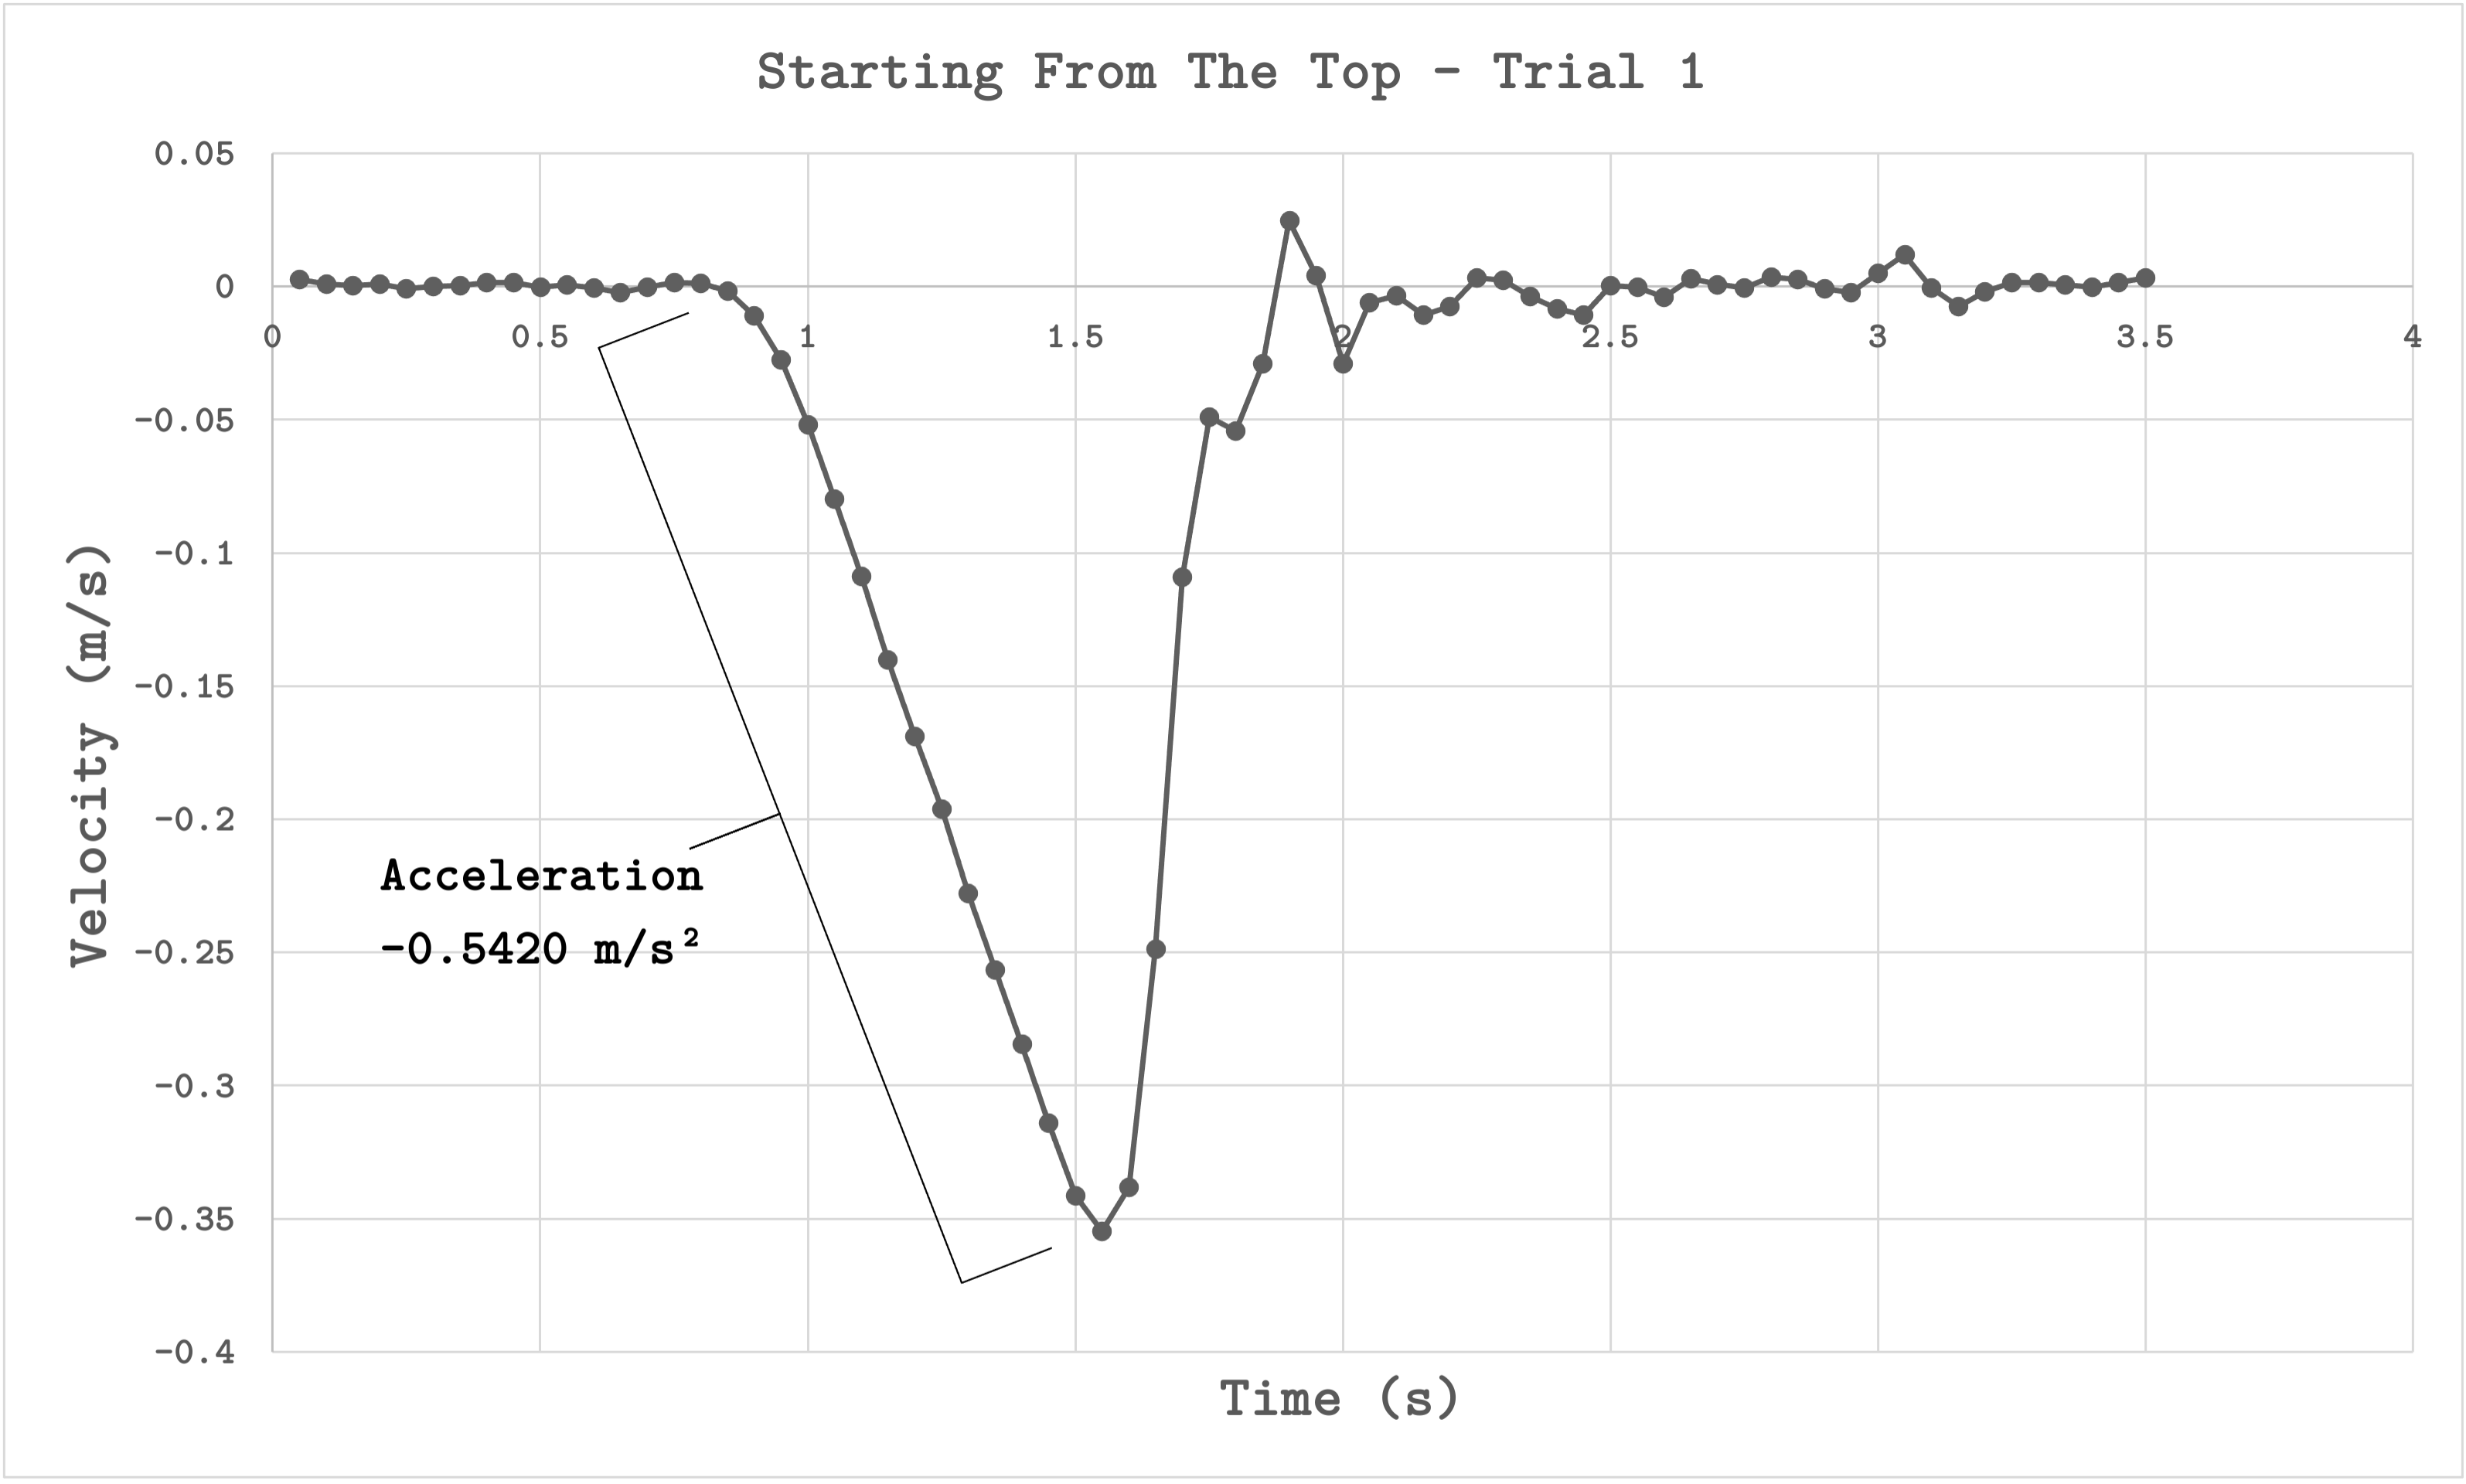
\includegraphics[width=0.95\textwidth]{cartg1.png}
	\end{center}
	\caption{Starting From The Top Graph | Trial 1}
	\label{fig:cartg1}
\end{figure} 
%----STARTING FROM THE TOP TRIAL 1-----%

%----STARTING FROM THE TOP TRIAL 1-4-----%
\subsubsection{Starting From The Top - Trials 1 - 4}

\begin{table}[H]
\centering
\begin{tabular}{@{}ccc@{}}
\toprule
\textbf{Trials} & \textbf{Acceleration} & \textbf{Relative Error (\%)} \\ \midrule
1 & -0.542 & 11.22 \\
2 & -0.5315 & 12.94 \\
3 & -0.529 & 13.34 \\
4 & -0.5244 & 14.1 \\ \midrule
\textbf{Average ($\boldsymbol{m/s^2}$)} & -0.5317 &  \\
\textbf{Standard Deviation ($\boldsymbol{m/s^2}$)} & 0.006455 &  \\ \bottomrule
\end{tabular}
\caption{Starting From The Top | Trials 1-4 }
\label{tab:ip-sftt}
\end{table}
%----STARTING FROM THE TOP TRIAL 1-4-----%

%----STARTING FROM THE BOTTOM TRIAL 1-----%
\subsubsection{Starting From The Bottom - Trial 1}
\begin{figure}[H]
	\begin{center}
		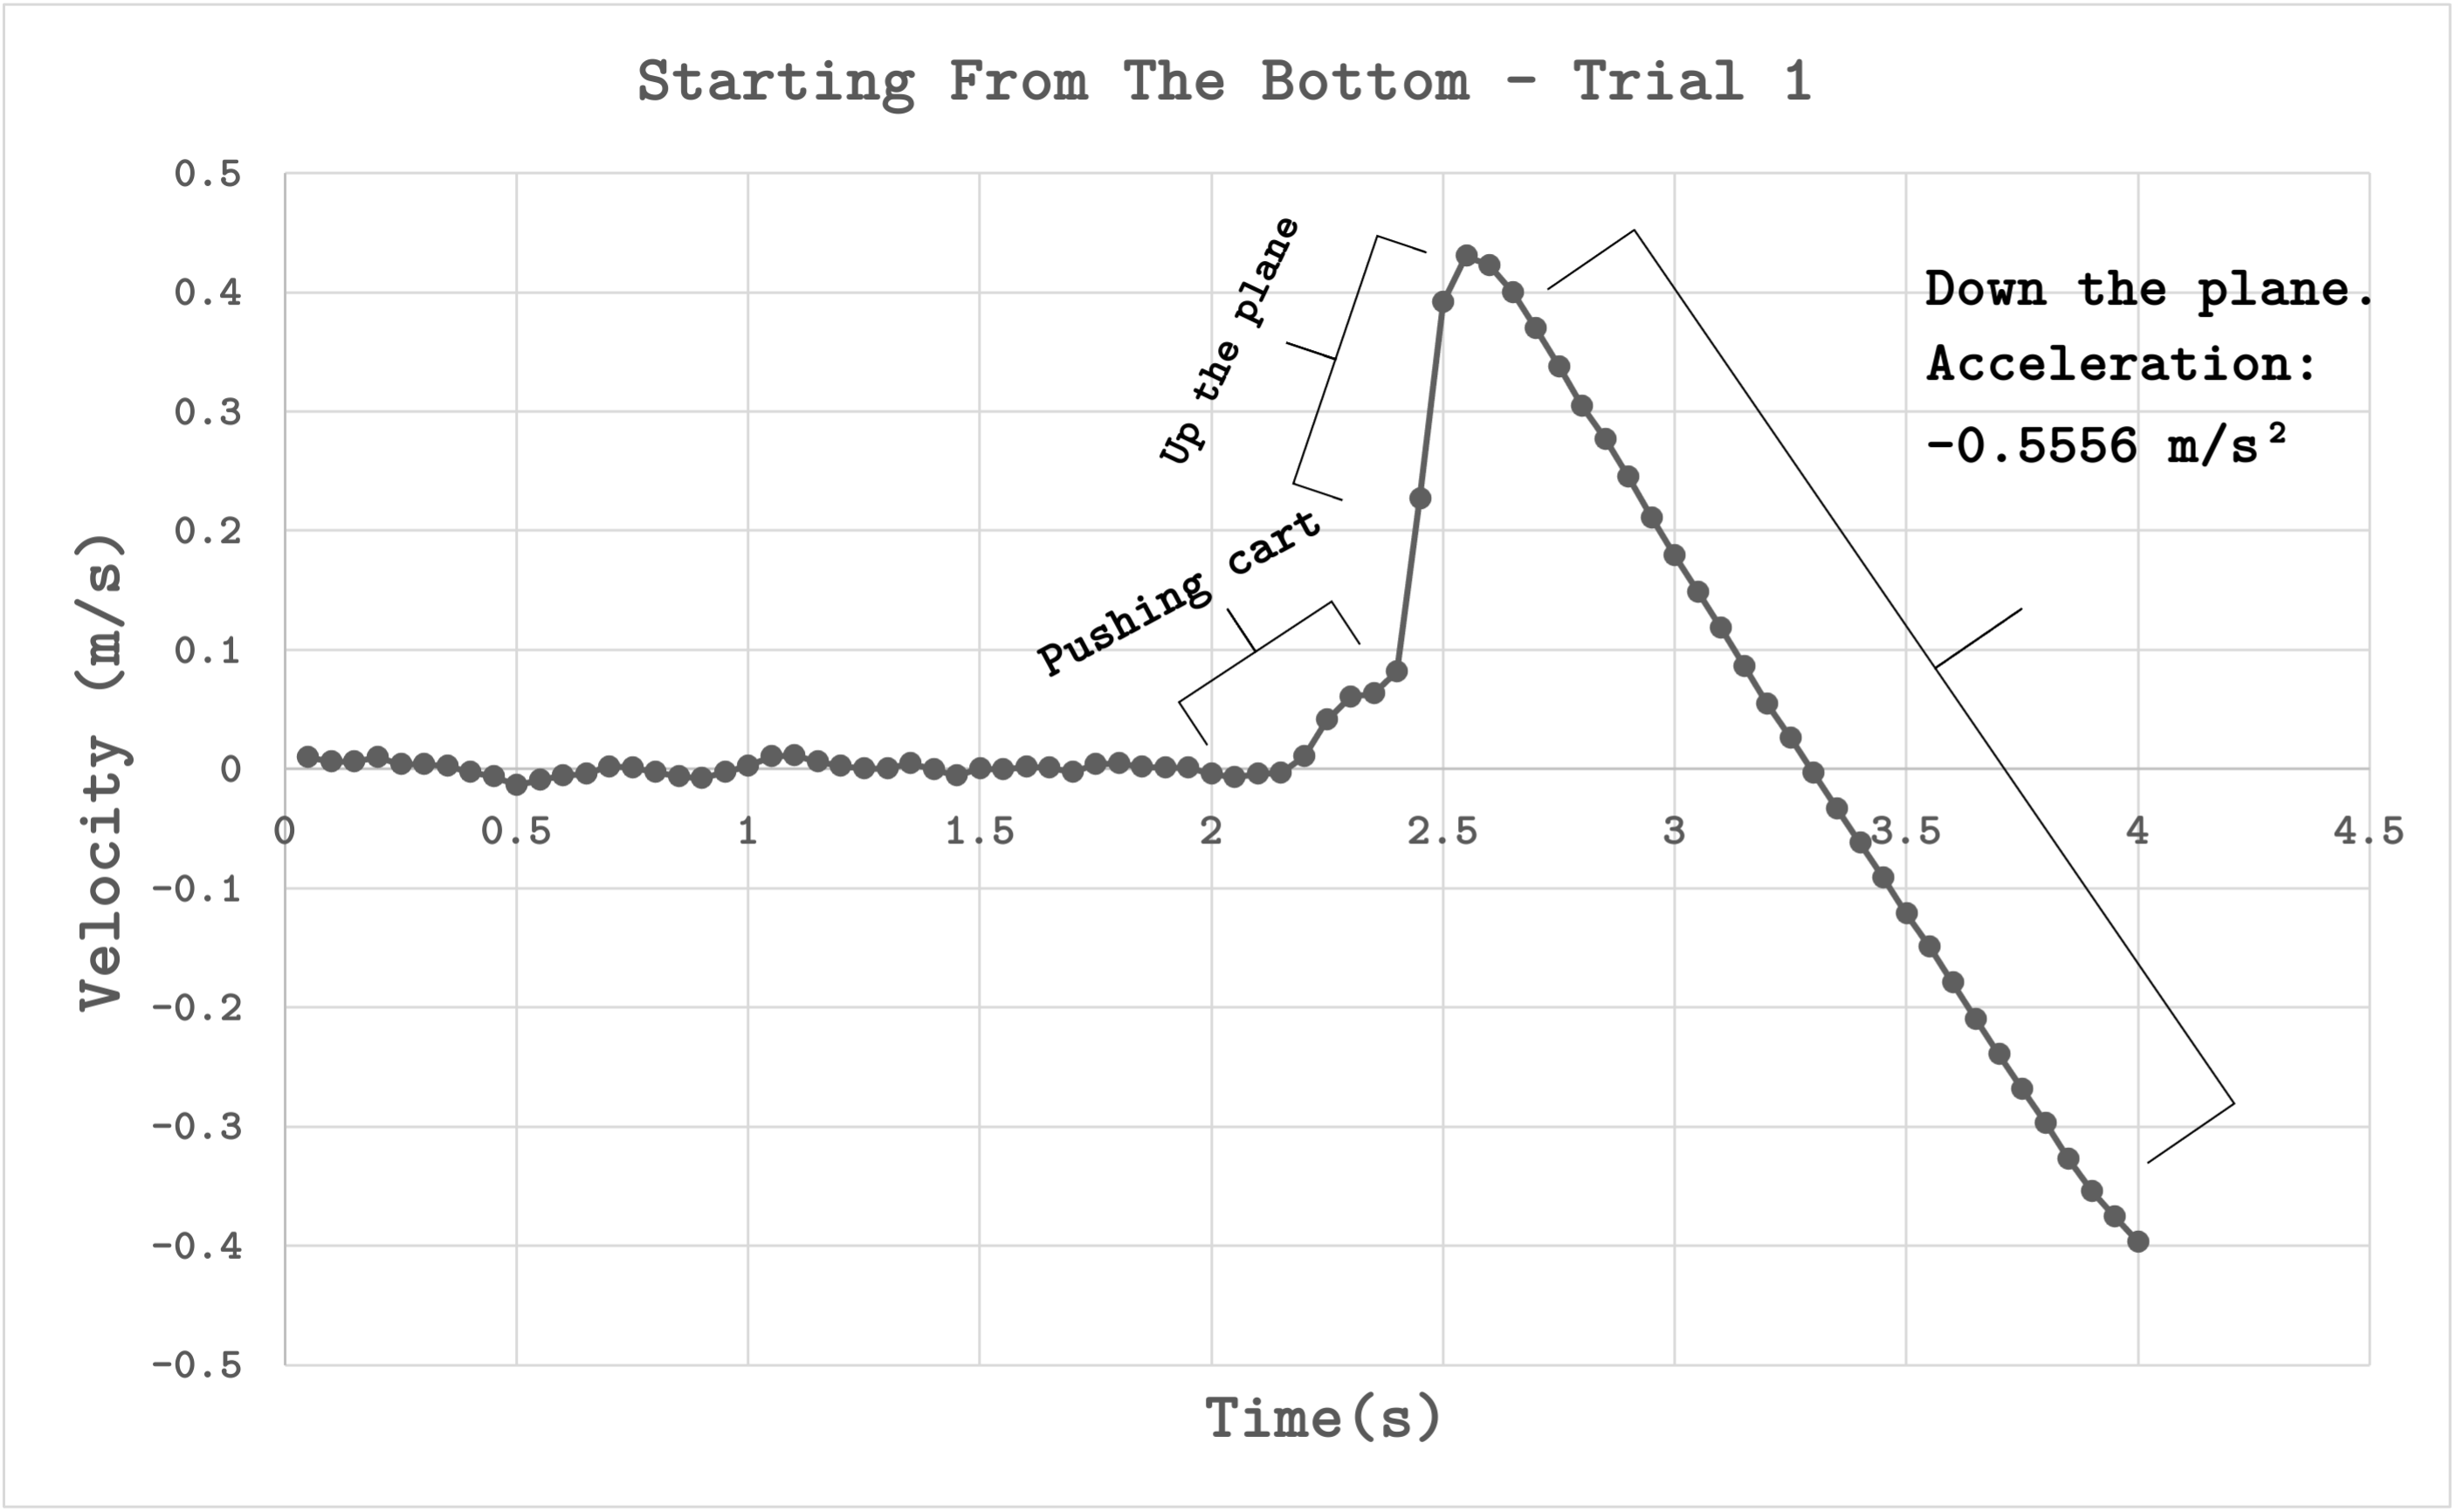
\includegraphics[width=0.95\textwidth]{cartg2.png}
	\end{center}
	\caption{Starting From The Bottom Graph | Trial 1}
	\label{fig:cartg2}
\end{figure} 

%----STARTING FROM THE BOTTOM TRIAL 1-----%

%----STARTING FROM THE BOTTOM TRIAL 1-4-----%
\subsubsection{Starting From The Bottom - Trials 1 - 4}

\begin{table}[H]
\centering
\begin{tabular}{@{}ccc@{}}
\toprule
\textbf{Trials} & \textbf{Acceleration} & \textbf{Relative Error (\%)} \\ \midrule
1 & -0.5556 & 8.992 \\
2 & -0.5755 & 5.733 \\
3 & -0.5622 & 7.911 \\
4 & -0.5639 & 7.633 \\ \midrule
\textbf{Average ($\boldsymbol{m/s^2}$)} & -0.5643 &  \\
\textbf{Standard Deviation ($\boldsymbol{m/s^2}$)} & 0.007171 &  \\ \bottomrule
\end{tabular}
\caption{Starting From The Bottom | Trials 1-4}
\label{tab:ip-sftb}
\end{table}
%----STARTING FROM THE BOTTOM TRIAL 1-----%

%----INCLINE PLANE AVERAGES RE-----%
\subsubsection{Incline Plane Averages - Relative Error}
\begin{table}[H]
\centering
\begin{tabular}{@{}ccc@{}}
\toprule
 & \textbf{Acceleration ($\boldsymbol{m/s^2}$)} & \textbf{Relative Error (\%)} \\ \midrule
\textbf{SFTT} & -0.5317 & 12.9 \\
\textbf{SFTB} & -0.5643 & 7.567 \\ \bottomrule

\end{tabular}
\caption{Inclined Plane Averages | Relative Error}
\label{tab:ip-re}
\end{table}
%----INCLINE PLANE AVERAGES RE-----%
